\begin{figure}[h!]
\begin{center}
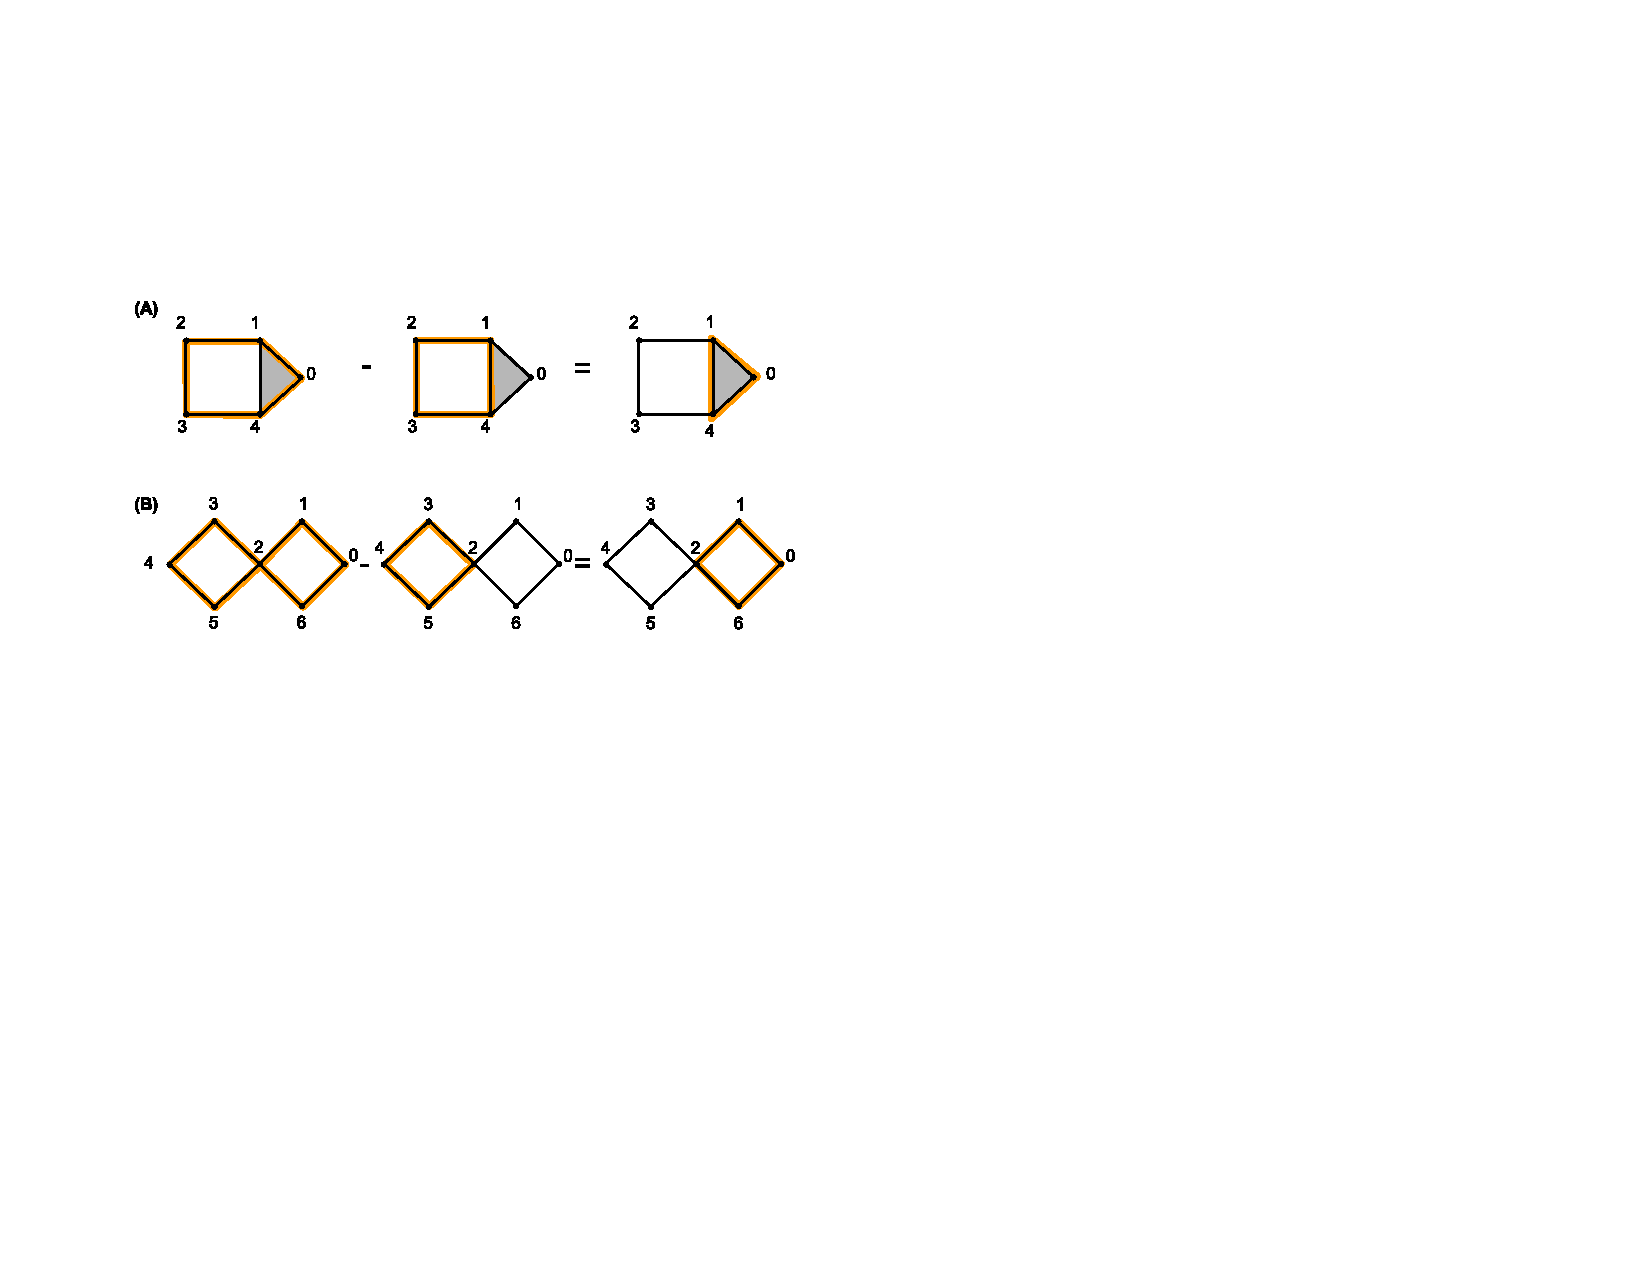
\includegraphics[width=1\textwidth]{figures/examplesorange.pdf}% This is a *.eps file
\end{center}
\caption{We show an example of homologous cycles in \textbf{(A)}, taken from \cite{TZH15}. The 1-cycle $(0,1) + (1,2) + (2,3) + (3,4) - (0,4)$ and the 1-cycle $(1,2) + (2,3) + (3,4) - (4,1)$ are homologous because their difference is the boundary of $(0,1,4)$. Subfigure \textbf{(B)} shows an example of non-homologous cycles. The 1-cycle $(\sum_{i=0}^4 (i, i+1))-(5,2)+(2,6)-(0,6)$ and the 1-cycle $(2,3) + (3,4)+(4,5)-(2,5)$ are not homologous because their difference is a cycle $(0,1)+(1,2)+(2,6)-(0,6)$ which is not a linear combination of boundaries of 2-simplices. } \label{fig:boundaryexample}
\end{figure}